
                \begin{figure}
                    \centering
                    \begin{tikzpicture}
                        \pgfplotsset{%
                            width=1\textwidth,
                            height=0.4\textheight
                        }
                        \begin{axis}[
                            xlabel={Runs since restart},
                            ylabel={Average dynamic energy (watt)},
                            ymin=0,ymax=70,
                        ]
                        
                            \addplot [mark=none, densely dashed, red]  coordinates {
                            (1, 0.11572768902380141)(2, 0.07419036983227956)(3, 0.07349316293494967)(4, 0.07677370000396333)(5, 0.07082352629836504)
                            };
                            \addlegendentry{WRK - IPG}
                            
                            \addplot [mark=none, densely dashed, blue]  coordinates {
                            (1, 0.09885066820980193)(2, 0.08395619890623067)(3, 0.0643557249508514)(4, 0.09757834508098547)(5, 0.0661934712859699)
                            };
                            \addlegendentry{WRK - LHM}
                            
                            \addplot [mark=none, densely dashed, cyan]  coordinates {
                            (1, 0.0)(2, 0.0)(3, 0.0)(4, 0.0)(5, 0.0)
                            };
                            \addlegendentry{WRK - CLAMP (win)}
                            
                        \end{axis}
                    \end{tikzpicture} 
                \caption{A graph illustrating the energy consumption of Dram for test case BinaryTrees with regards to how long ago the DUT was restarted, experiment \#2, (with outliers)} \label{fig:BinaryTrees_Dram_iteration_exp2}
                \end{figure}
                